\documentclass[./dokumentation.tex]{subfiles}

\begin{document}
\chapter{Verwendung vom Emotionen im Design}
Große Bilder (z.B.: Darstellungen von Personen vergrößern, nah an den Rahmen heranrücken), leuchtende Farben mit hoher Sättigung und hohe Kontraste auf Webseiten wirken erregender auf den Nutzer und können somit ein besonders wirkungsvoller Kanal sein, Aufmerksamkeit zu erhöhen und das Verhalten zu beeinflussen. Dabei erfolgt die Erregung größtenteils unbewusst und bietet somit für die Webdesigner einen besonders wirkungsvollen Kanal. Denn eine erhöhte Erregung verengt den Fokus der Aufmerksamkeit, sodass sich diese auf das richtet,  was die Stimulation (Erregung) verursacht (z.B.: Stoppschild) \cite{vanGorp2013}. 

\section{Motivation und Emotionen}
Emotionen beeinflussen das Verhalten der Nutzer. Beispielsweise vermeiden die Nutzer Produkte, die sie mit negativen Emotionen (z.B.: Schmerz) verbinden und suchen eher Nähe zu Produkten, die sie mit positiven Gefühlen (z.B.: Freude) verbinden. Wie sehr die Nutzer durch eine Webseite erregt werden, hat Einfluss auf deren Motivation. Dabei können sowohl Angst als auch Aufregung starke Erregung hervorrufen. Je intensiver eine Emotion ist, desto mehr Aufmerksamkeit fordert diese und beeinflusst auch unsere Motivation. Geringe Angst oder Langeweile führen zu einer geringen Motivation und somit auch wenig Handlung. Dabei ist zu beachten, dass große Angst zwar zu einer höheren Motivation führt, diese jedoch nur bis zu einem bestimmten optimalen Niveau, diese Wirkung hat und bei weiterer Zunahme dann eher zu Handlungsfähigkeit und geringer Motivation führt \cite{vanGorp2013}.

\section{Motivation und Emotionen}
Als soziale Wesen nehmen Menschen den Ausdruck von Emotionen in allem wahr, auch auf Webseiten oder Objekten. Ein Beispiel ist in Abbildung 3 zu sehen. Hierbei geschieht eine Zuweisung von Persönlichkeiten auf Grundlage der Art und Weise, wie z.B.: Webseiten die Sinne von Nutzern ansprechen. Beziehungen die durch Verwendung von Produkten entstehen können Menschen z.B.: glücklich oder traurig, passiv, entspannt, wütend oder motiviert machen \cite{vanGorp2013}. \\


\begin{figure}[h]
    \centering
    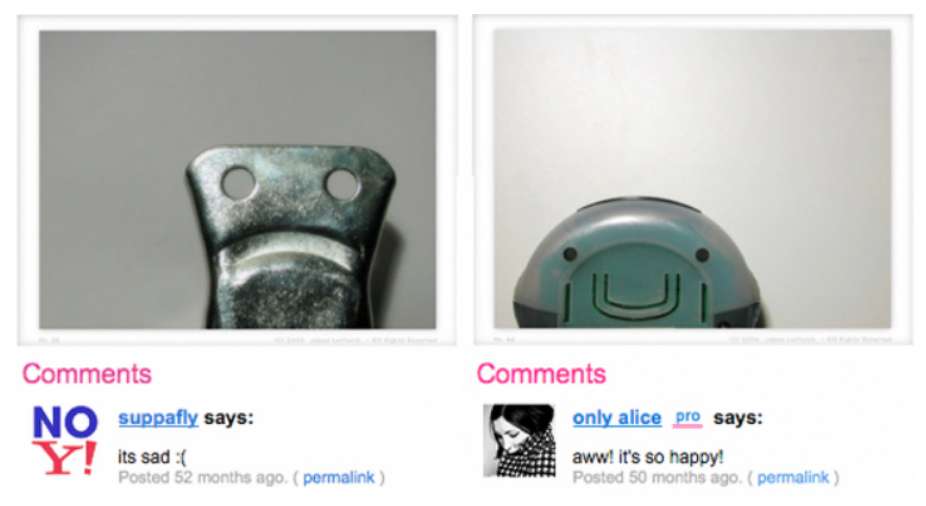
\includegraphics[width=0.8\textwidth]{bilder/sad-happy.png}
    \caption{Beispiele für die Zuweisung von Emotionen und Persönlichkeiten zu Objekten}
    \label{fig6:happy}
\end{figure}\\

Auch Eigenschaften, wie Dominanz und Unterwürfigkeit können über visuelle Merkmale vermittelt werden. Dabei wird Dominanz vor allem durch kalte/kühle oder dunkle Farben, wie schwarz oder silber, vermittelt. Auch eckige oder gerade Formen tragen dazu bei. Unterwürfige Gestaltung geschieht vor allem durch runde Formen und helle, klare, warme, zarte oder weiche Formen und Farben/Farbübergänge \cite{DesignEmo2003}. Allgemein kann gesagt werden, dass sich Personen von den Webseiten eher angesprochen fühlen, deren visuelle Persönlichkeit der eigenen Persönlichkeit oder der Persönlichkeit, die wir gern darstellen wollen, am nächsten kommt. Somit kann die Anziehung einer bestimmten Webseite von Nutzergruppe zu Nutzergruppe stark schwanken \cite{vanGorp2013}. \\

\begin{figure}[h]
    \centering
    
\includegraphics[width=0.8\textwidth]{bilder/dom.png}
    \caption{Beispiel für eine dominante Gestaltung \cite{dom_bsp}}
    \label{fig7:dom}
\end{figure}\\

\begin{figure}[h]
    \centering
    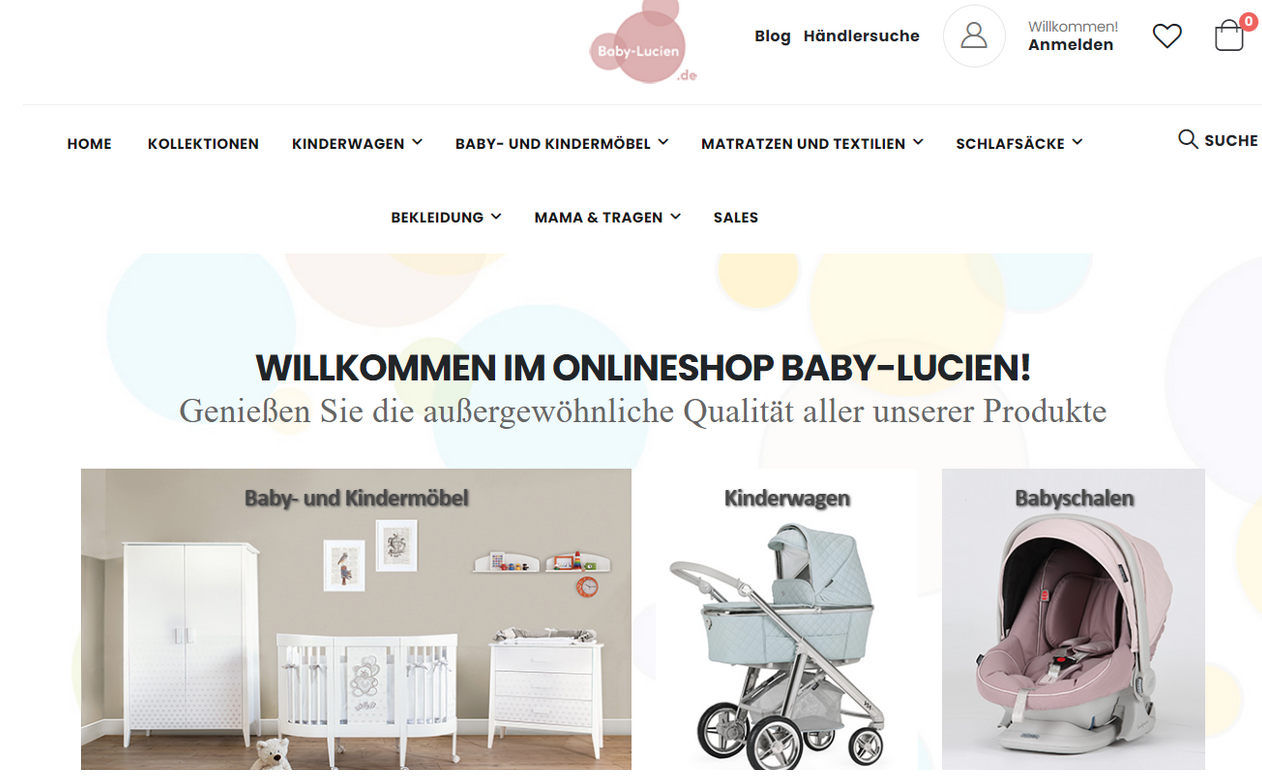
\includegraphics[width=0.8\textwidth]{bilder/unt.png}
    \caption{Beispiel für eine devote Gestaltung \cite{unt_bsp}}
    \label{fig8:unt}
\end{figure}\\
\section{Angst, Überraschung, Wut}
Wenn Angst empfunden wird, zeigt dies häufig, dass es sich um eine dringliche Ausnahmesituation handelt. Angst ist ein natürlicher Instinkt und zeigt, dass gehandelt werden muss, um Beispielsweise Überlebenschancen zu erhöhen. In der Werbung wird Angst oft genutzt, um Botschaften einzuprägen und den Kunden zu vermitteln, dass sie jetzt handeln müssen, um etwas zu verändern bzw. zu kaufen, um vor Dingen beschützt zu werden, die sonst eintreten könnten. Hierbei muss jedoch beachtet werden, dass bestimmte Grenzen gewahrt werden müssen, damit beispielsweise eine Webseite auf den Nutzer nicht abschreckend oder verstörend wirkt.
Wut, als negatives Gefühl, kann ebenfalls sehr Wirksam 
sein. Wird diese richtig platziert, ist es möglich, Nutzer “aufzuwecken” und ebenfalls zum Handeln zu bewegen, denn auch diese Emotion birgt hohes Motivationspotenzial. Empörung und Frustration können einen Perspektivwechsel erzwingen und eine Auseinandersetzung mit einer Thematik erzwingen  \cite{Schubert2016}.



\end{document}


